\subsection{Rappel sur le maximum de vraisemblance}

En statistique paramétrique, on suppose qu'un ensemble d'observations $\mathbf{X}$ est la réalisation d'une variable aléatoire dont la loi dépend d'un ensemble de paramètres $\theta$ inconnu. 
L'inférence statistique consiste en la définition d'un estimateur de $\theta$.

Un estimateur générique commun est l'estimateur du maximum de vraisemblance. 

Le modèle statistique posé permettant d'écrire la loi de $\mathbf{X}$ quand on connaît $\theta$, que l'on note $L(\mathbf{X}, \theta)$. 
On choisit comme estimateur le paramètre $\hat{\theta}$ \textit{le plus vraisemblable}, c'est à dire celui qui maximise (en $\theta$) la fonction $L(\mathbf{X}, \theta)$.

L'estimateur du maximum de vraisemblance pour \(\mathbf{X}\) est donné
par
\(\hat{\theta} = \text{argmax}_{\theta}L(\theta\vert \mathbf{X}) = \frac{\sum_{i=1}^n X_i}{n}\).

Cet estimateur \textbf{est une variable aléatoire}. Sa loi dépend du modèle, mais 
asymptotiquement, un thérème central limite nous assure que sa distribution devient celle d'une loi Normale (dont l'expression de la variance est connue, au moins en théorie).

Dans ce contexte, le paramètre $\theta$ est donc une quantité fixe inconnue. Toute la connaissance sur sa valeur vient des données.

\subsection{Inférence bayésienne}

\subsubsection{Connaissance a priori et définition du posterior}

Dans le contexte de l'inférence bayésienne, on supposera que le paramètre $\theta$ est lui même aléatoire.
On modélisera alors sa loi sous la forme d'une distribution. Cette distribution est indépendante des données et s'appelle la distribution \textit{a priori}. 
Elle reflète la connaissance (et l'incertitude) que l'on a sur le paramètre.
La loi a priori sur $\theta$ sera notée  $\pi(\theta)$.

L'objectif de l'inférence bayésienne est d'actualiser cette connaissance (et son incertitude) grâce au données. La quantité d'intérêt, dans ce contexte est alors la loi de $\theta\vert \mathbf{X}$, quand appelle loi a posteriori (ou posterior). Cette quantité sera notée 
$\pi(\theta \vert \mathbf{X})$.

La formule de Bayes sur le conditionnement permet de lier cette loi a posteriori à la loi a priori et à la vraisemblance du modèle:

$$\pi(\theta\vert \mathbf{X}) = \frac{\pi(\theta)L(\mathbf{X}\vert \theta)}{\int \pi(u)L(\mathbf{X}\vert u} d u$$


Ce sont les caractéristiques de cette loi (ses quantiles, ses moments) que l'on cible dans ce contexte. 

\textbf{L'objectif de l'inférence bayésienne est donc la détermination de $\pi(\theta\vert \mathbf{X})$}.

\subsubsection{Estimateurs bayésiens}

Les estimateurs bayésiens sont des quantités liées à la loi à posteriori.

On mentionnera:

\begin{itemize}
\end{itemize}


% 
% \subsection{Simple modèle paramétrique}
% 
% \subsubsection{Expérience et question}
% 
% Supposons que l'on observe n = 10 tirages indépendant de pile ou face.
% On compte 8 observations de piles et 2 de faces.
% 
% Quelle est la probabilité que la pièce tombe sur pile?
% 
% \subsubsection{Modélisation}
% 
% On suppose qu'on a 10 V.A. \(X_1,\dots,X_{10}\) i.i.d. de loi
% \(\mathcal{B}ern(\theta)\) où \(\theta \in ]0, 1[\) est la probabilité
% d'obtenir pile.
% 
% Donc, la loi jointe de \(\mathbf{X} = (X_1,\dots,X_{n})\) est donnée
% par:
% \[f(\mathbf{X}\vert \theta) = \prod_{i = 1}^{n}\mathbb{P}(X = X_i)\] où
% \(X \sim \mathcal{B}ern(\theta)\).
% 
% \subsection{Inférence par maximum de vraisemblance}
% 
% Pour un échantillon \(\mathbf{X} = X_1, \dots, X_n\), et pour un
% paramètre \(\theta \in ]0, 1[\), la \emph{vraisemblance} de \(\theta\)
% est:
% \[L(\theta \vert \mathbf{X}) := f(\mathbf{X}\vert \theta) = \theta^{\sum_{i=1}^n X_i}\left(1 - \theta \right)^{n - \sum_{i=1}^n X_i}.\]
% La courbe de vraisemblance pour le modèle et les proportions décrites plus haut est montrée sur la figure \ref{fig:beta:bin:vraisemblance}, pour $n = 10$ et $n = 1000$.
% 
% \begin{figure}[ht]
% \centering
% \label{fig:beta:bin:vraisemblance}
% \begin{tabular}{cc}
% 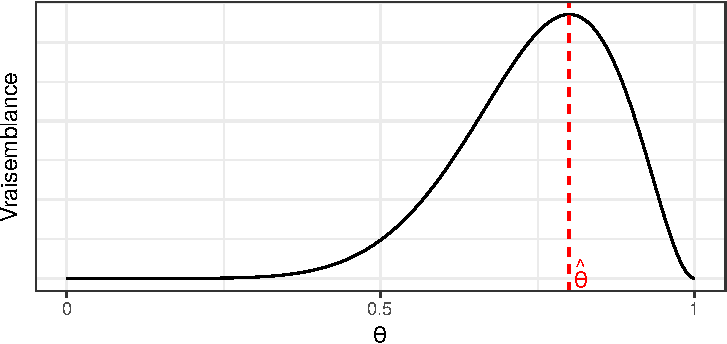
\includegraphics[width = 0.45\textwidth]{figures/vraisemblance_10.pdf} &
% 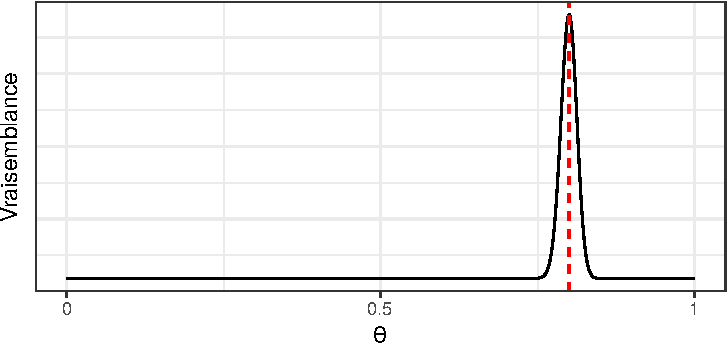
\includegraphics[width = 0.45\textwidth]{figures/vraisemblance_1000.pdf} 
% \end{tabular}
% \end{figure}
% 
% \subsubsection{Maximum de vraisemblance}
% 
% L'estimateur du maximum de vraisemblance pour \(\mathbf{X}\) est donné
% par
% \(\hat{\theta} = \text{argmax}_{\theta}L(\theta\vert \mathbf{X}) = \frac{\sum_{i=1}^n X_i}{n}\).
% 
% L'estimateur est \textbf{entièrement basé sur les données}.
% 
% \subsubsection{Incertitude sur $\theta$}
% 
% \(\hat{\theta}\) est une variable aléatoire. 
% La théorie du MLE nous dit que cet estimateur admet un TCL.
%  Ainsi, \emph{asymptotiquement}, on a toujours un intervalle de confiance pour \(\theta\).
% 
% 
% \subsection{Inférence bayésienne}
% 
% \subsubsection{A priori sur $\theta$}
% 
% On a potentiellement une connaissance \emph{a priori} sur \(\theta\). On peut modéliser cet \emph{a priori} sur le paramètre \(\theta\) (savoir expert\ldots{}) par une \textbf{variable aléatoire} de densité
% \(\pi(\theta)\). 
% Cette distribution est appelée \textbf{prior} sur \(\theta\).

% \begin{center}\includegraphics{intro_bayes_files/figure-latex/plot_prior-1} \end{center}

%\hypertarget{inference-bayesienne-1}{%
%\subsection{Inférence bayésienne}\label{inference-bayesienne-1}}
%
%\hypertarget{influence-des-donnees-distribution-a-posteriori.}{%
%\subsubsection{Influence des données, distribution a
%posteriori.}\label{influence-des-donnees-distribution-a-posteriori.}}
%
%En inférence bayésienne, l'objectif est de connaître la distribution de
%\(\theta\) \textbf{sachant les données} \(\mathbf{x}\). Cette densité
%sur \(\theta\) est notée \(\pi(\theta \vert \mathbf{x})\), et est
%appelée \textbf{posterior}.
%
%\hypertarget{formule-de-bayes}{%
%\subsubsection{Formule de Bayes}\label{formule-de-bayes}}
%
%\[
%\pi(\theta \vert \mathbf{x}) = \frac{f(\mathbf{x}, \theta)}{f(\mathbf{x})} = \frac{f(\mathbf{x} \vert \theta)\pi(\theta)}{f(\mathbf{x})}
%\] où \(f\) est notation surchargée pour les densités.
%
%Cette relation est résumée par:
%\[\pi(\theta \vert \mathbf{x}) \propto f(\mathbf{x} \vert \theta)\pi(\theta)\]
%
%\hypertarget{objectif-de-linference-bayesienne}{%
%\subsubsection{Objectif de l'inférence
%Bayésienne}\label{objectif-de-linference-bayesienne}}
%
%L'inférence Bayésienne a pour but la détermination (exacte, ou par
%simulation) du posterior \(\pi(\theta\vert \mathbf{x})\).
%
%\hypertarget{posterior-pour-un-prior-betaa-b}{%
%\subsection{\texorpdfstring{Posterior pour un prior
%\(\beta(a, b)\)}{Posterior pour un prior \textbackslash{}beta(a, b)}}\label{posterior-pour-un-prior-betaa-b}}
%
%Dans ce cas, on a \(\pi(\theta\vert \mathbf{x})\) est la densité d'une
%loi \[\beta\left(a + \sum_{i}^n x_i, b + n - \sum_{i}^n x_i\right)\]
%
%\hypertarget{cas-n-10-et-8-succues}{%
%\subsubsection{\texorpdfstring{Cas \(n = 10\) et 8
%succès}{Cas n = 10 et 8 succès}}\label{cas-n-10-et-8-succues}}
%
%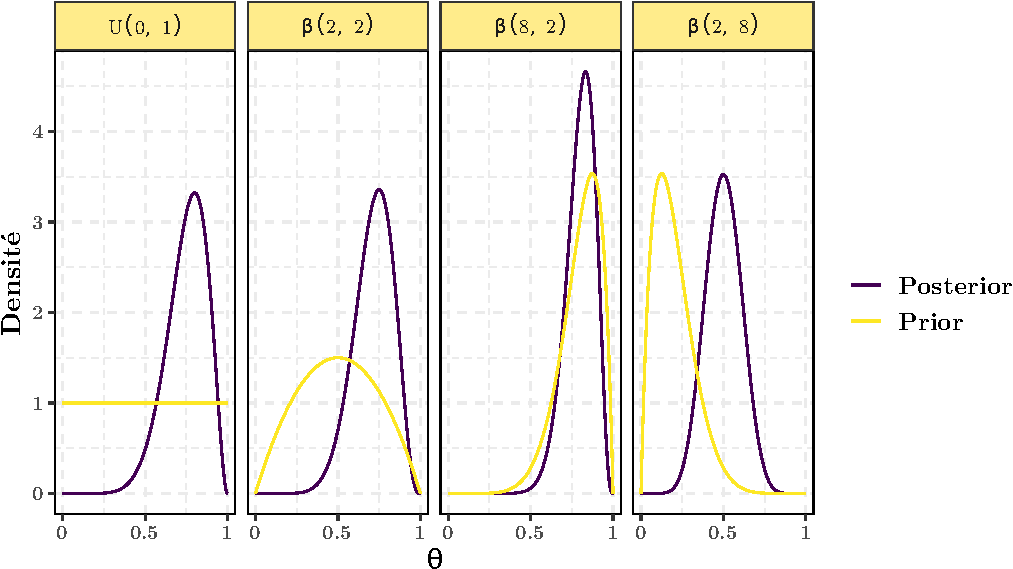
\includegraphics{intro_bayes_files/figure-latex/plot_prior_posterior_small_samp-1.pdf}
%
%\hypertarget{posterior-pour-un-prior-betaa-b-1}{%
%\subsection{\texorpdfstring{Posterior pour un prior
%\(\beta(a, b)\)}{Posterior pour un prior \textbackslash{}beta(a, b)}}\label{posterior-pour-un-prior-betaa-b-1}}
%
%Dans ce cas, on a \(\pi(\theta\vert \mathbf{x})\) est la densité d'une
%loi \[\beta\left(a + \sum_{i}^n x_i, b + n - \sum_{i}^n x_i\right)\]
%
%\hypertarget{cas-n-1000-et-800-succues}{%
%\subsubsection{\texorpdfstring{Cas \(n = 1000\) et 800
%succès}{Cas n = 1000 et 800 succès}}\label{cas-n-1000-et-800-succues}}
%
%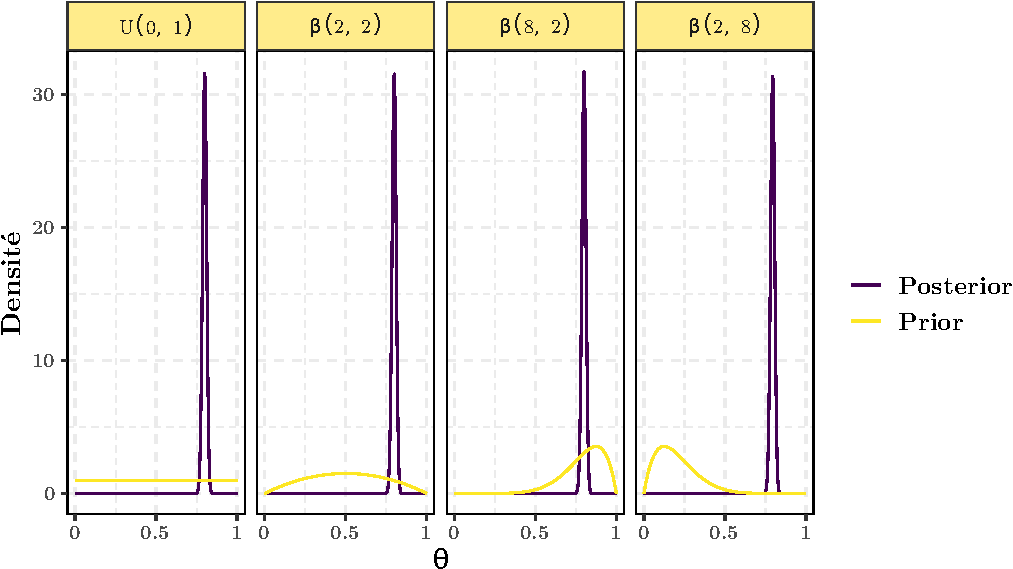
\includegraphics{intro_bayes_files/figure-latex/plot_prior_posterior_large_samp-1.pdf}
%
%\hypertarget{estimateurs-bayesiens}{%
%\subsection{Estimateurs Bayésiens}\label{estimateurs-bayesiens}}
%
%\hypertarget{esperance-a-posteriori}{%
%\subsubsection{Espérance a posteriori}\label{esperance-a-posteriori}}
%
%Soit un modèle Bayésien paramétré par une vraie valeur
%\(\theta^* \in \Theta\) et de prior \(\pi(\theta)\) Pour toute fonction
%\(\varphi\), la variable aléatoire
%\[\mathbb{E}[\varphi(\theta) \vert \mathbf{X}]\] est un estimateur
%Bayésien de \(\varphi(\theta^*)\).
%
%Par exemple, pour un échantillon observé \(\mathbf{x}\), l'estimation
%bayésienne de \(\theta^*\) est
%\[\hat{\theta}^* = \mathbb{E}[\theta \vert \mathbf{X} = \mathbf{x}] = \int_\Theta \theta \pi(\theta \vert \mathbf{x}) \text{d}\theta\]
%
%\hypertarget{exemple-sur-la-moduele-bernouilli-beta}{%
%\subsubsection{Exemple sur la modèle
%Bernouilli-Beta}\label{exemple-sur-la-moduele-bernouilli-beta}}
%
%Pour un prior \(\beta(a, b)\), on a
%\[\hat{\theta}^* \overset{\text{loi } \beta}{=} \frac{a + \sum_{i = 1}^n x_i}{a + b + n} = \underbrace{\frac{n}{a + b + n}}_{\text{Poids données}}\times \overbrace{\frac{\sum_{i=1}^n x_i}{n}}^{\text{Max. de vrais.}} + \underbrace{\frac{a + b}{a + b + n}}_{\text{Poids prior}} \times \overbrace{\frac{a}{a + b}}^{\mathbb{E}\text{ du prior}}\]
%
%\hypertarget{estimateurs-bayesiens-1}{%
%\subsection{Estimateurs Bayésiens}\label{estimateurs-bayesiens-1}}
%
%\hypertarget{intervalle-de-credibilite}{%
%\subsubsection{Intervalle de
%crédibilité}\label{intervalle-de-credibilite}}
%
% Pour toute région \(\mathcal{R} \subset \Theta\), on peut quantifier:
% \[\mathbb{P}(\theta \in \mathcal{R} \vert  \mathbf{X} = \mathbf{x}) = \int_\mathcal{R} \pi(\theta \vert \mathbf{x}) \text{d}\theta\]
% Pour \(\alpha \in ]0, 1[\), une région de crédibilité de niveau
% \(1-\alpha\) est une région \(\mathcal{R} \subset \Theta\) telle que
% \[\mathbb{P}(\theta \in \mathcal{R} \vert  \mathbf{X} = \mathbf{x}) = 1 - \alpha\]
% Cet intervalle n'est pas asymptotique, mais \textbf{dépend du prior}
%
%\hypertarget{intervalles-de-credibilites-centres-uxe0-95-dans-bernouilli-beta}{%
%\subsection{Intervalles de crédibilités (centrés) à 95\% dans Bernouilli
%Beta}\label{intervalles-de-credibilites-centres-uxe0-95-dans-bernouilli-beta}}
%
%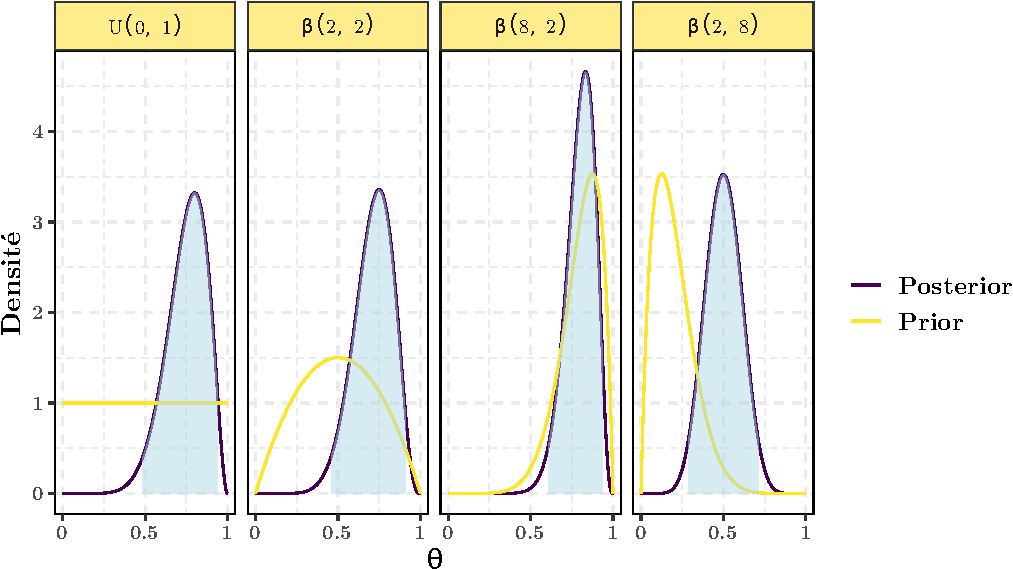
\includegraphics{intro_bayes_files/figure-latex/intervalle_credi-1.pdf}
%
%\hypertarget{influence-et-choix-du-prior}{%
%\subsection{Influence et choix du
%prior}\label{influence-et-choix-du-prior}}
%
%On a vu que pour un nombre de données limité, la \textbf{forme du prior}
%a un impact sur la forme du posterior.
%
%\hypertarget{choix-du-prior}{%
%\subsubsection{Choix du prior}\label{choix-du-prior}}
%
%La forme du prior peut être choisie en fonction du \emph{savoir expert}
%(littérature existante, expériences passées).
%
%\textbf{ATTENTION} Le support du posterior sera toujours inclu dans le
%support du prior.
%
%Si le prior charge également tout le support, on dit qu'il est
%\textbf{non informatif}.
%
%\hypertarget{prior-impropre}{%
%\subsubsection{Prior impropre}\label{prior-impropre}}
%
%Si le support de \(\theta\) est sur \(\mathbb{R}\), un prior non
%informatif est une ``uniforme sur \(\mathbb{R}\)''. Ceci n'est pas une
%loi. On peut cependant noter abusivement \(\pi(\theta) \propto 1\).
%
%Pour autant, si
%\(\frac{f(\mathbf{x} \vert \theta)}{\int f(\mathbf{x\vert \theta})\text{d} \theta}\)
%définit une loi de probabilité en \(\theta\), alors le posterior
%\(\pi(\theta\vert \mathbf{x})\) est bien défini. Dans ce cas, le prior
%est dit \textbf{impropre}.
%
%\hypertarget{choix-du-prior-1}{%
%\subsection{Choix du prior}\label{choix-du-prior-1}}
%
%\hypertarget{exemple-de-prior-impropre.}{%
%\subsubsection{Exemple de prior
%impropre.}\label{exemple-de-prior-impropre.}}
%
%On suppose que \(\mathbf{x}\) est issu d'un échantillon i.i.d. de taille
%\(n\), de loi \(\mathcal{N}(\mu, 1)\) où \(\mu\) est inconnu. N'ayant
%aucune idée de la valeur de \(\mu\), on prend un prior non informatif.
%On a alors: \begin{align*}
%\pi(\mu \vert \mathbf{x}) &\propto f(\mathbf{x} \vert \theta)\\
%&\propto \text{e}^{-\frac{1}{2}\sum_{i = 1}^n (x_i - \mu)^2}\\
%&\propto\text{e}^{-\frac{1}{2}(n \mu - 2\mu\sum_{i = 1}^n x_i)}\\
%&\propto\text{e}^{-\frac{n}{2}(\mu - \frac{1}{n}\sum_{i = 1}^n x_i)^2}
%\end{align*} Ainsi,
%\(\mu\vert \mathbf{x} \sim \mathcal{N}\left(\frac{1}{n}\sum_{i = 1}^n x_i, \frac{1}{n}\right)\)
%
%\hypertarget{prior-conjugue}{%
%\subsection{Prior conjugué}\label{prior-conjugue}}
%
%Pour les modèles basés sur une vraisemblance ``classique'', certains
%priors ont des priorités de conjugaison. Pour un modèle Bayésien, on
%appelle prior conjugué un prior \(\pi(\theta)\) tel que le posterior
%\(\pi(\mathbf{x}\vert \theta)\) est dans la même famille de loi que
%\(\pi(\theta)\).
%
%\hypertarget{exemples}{%
%\subsubsection{Exemples}\label{exemples}}
%
%\begin{itemize}
%\tightlist
%\item
%  Modèle Bernouilli-Beta;
%\item
%  Modèle Gaussien (prior: Normal Inverse Gamma);
%\item
%  Modèle à densités dans la famille exponentielle.
%\end{itemize}
%
%\hypertarget{interuxeat}{%
%\subsubsection{Intérêt}\label{interuxeat}}
%
%L'inférence est directe!
%
%\hypertarget{cas-generique-un-posterior-de-densite-non-standard}{%
%\subsection{Cas générique, un posterior de densité non
%standard}\label{cas-generique-un-posterior-de-densite-non-standard}}
%
%Dans la majorité des modèles, le produit
%\(\pi(\theta \vert \mathbf{x}) \propto f(\mathbf{x} \vert \theta) \pi(\theta)\)
%n'a aucune raison d'être dans une densité connue.
%
%Dans ces cas, le calcul d'espérances a posteriori est impossible.
%
%On aura recours à des méthodes de Monte Carlo pour les approcher. Les
%méthodes les plus utilisées sont les MCMC.
